% !TeX encoding = UTF-8
% !TeX spellcheck = en_US
% !TeX root = main.tex

%% Chapter03-机载LiDAR数据获取基本原理.tex
\chapter{机载LiDAR数据获取基本原理} %% Chapter 机载LiDAR数据获取基本原理

\paragraph{机载LiDAR系统工作原理}如图\ref{fig:机载LiDAR系统工作原理图}所示。
\begin{figure}[htbp]
	\centering
	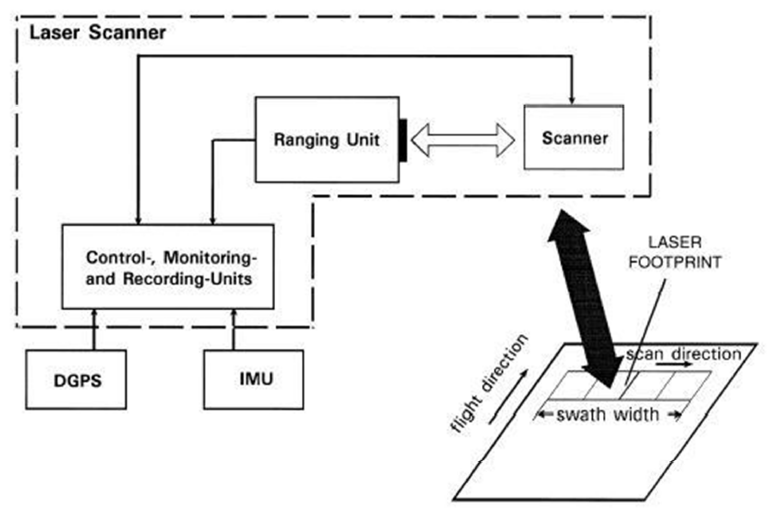
\includegraphics[width=0.7\linewidth]{figure/Chapter3/机载LiDAR系统工作原理图}
	\caption{机载LiDAR系统工作原理图}
	\label{fig:机载LiDAR系统工作原理图}
\end{figure}

图中,
\begin{itemize}
	\item \textit{激光测距单元}包括:激光发射器和接收机。
	\item 光学机械扫描装置:主动工作方式。
		\begin{itemize}
			\item 激光发射器产生激光,由扫描装置控制激光束发射出去的方向
			\item 扫描方向一般与飞机飞行方向垂直。
			\item 扫描宽度由\textit{扫描视场}(FOV,field of view)决定。
		\end{itemize}
	\item 发射和接收激光束的光孔是同一光孔,孔径一般为8$ \sim $15 cm,保证发射光路和接收光路是同一光路。
	\item 发射的激光束是一束很窄的光,发散度很小,形成的\textit{瞬时视场}(IFOV,instantaneons field of view)是由一个很小的角度确定的,一般为0.3 毫弧(mrad)到0.2 毫弧,激光束形成的一个照射角,照射在一小块地面。
	\item 接收机接收被反射回来的激光束后由记录单元进行记录。
\end{itemize}

\paragraph{关键技术}
\begin{itemize}
	\item 激光测距技术
	\item 全球定位系统技术
	\item 惯性测量系统技术
	\item 高性能二维扫描技术
\end{itemize}

\section{激光测距} %% Section	激光测距	========================================
\paragraph{机载LiDAR系统对测距仪的要求}
\begin{itemize}
	\item 精度高
	\item 功率高
	\item 体积小
	\item 波长合适
\end{itemize}

\paragraph{激光测距基本原理}测量激光往返目标所需要时间,然后通过光速$ c $(299792458 m/s)和大气折射系数计算出距离。如图\ref{fig:激光测距基本原理}所示。
\begin{figure}[htbp]
	\centering
	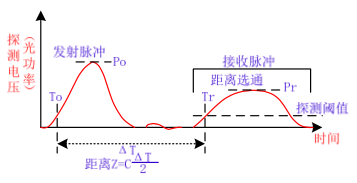
\includegraphics[width=0.7\linewidth]{figure/Chapter3/激光测距基本原理}
	\caption{激光测距基本原理}
	\label{fig:激光测距基本原理}
\end{figure}

\subsection{测距方式} % Subsection	测距方式	----------------------------------------
\paragraph{脉冲测距}
\begin{enumerate}
	\item \textbf{测距原理}:发射脉冲波,测量脉冲信号往返时间差,如图\ref{fig:脉冲测距原理}所示。距离为
		\begin{equation}
		R = \dfrac{1}{2}ct_L
		\end{equation}
		\begin{figure}[htbp]
			\centering
			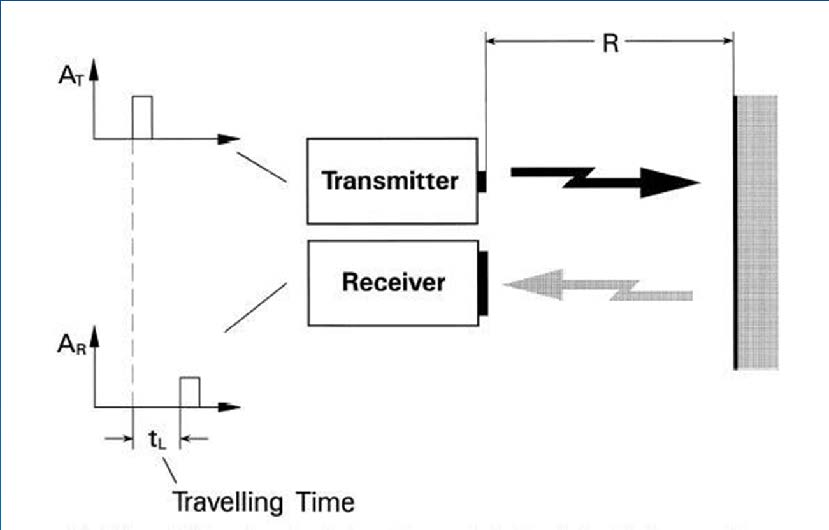
\includegraphics[width=0.5\linewidth]{figure/Chapter3/脉冲测距原理}
			\caption{脉冲测距原理}
			\label{fig:脉冲测距原理}
		\end{figure}
	\item \textit{测距分辨率}:在光束方向能够区分的两个物体的最小距离。
		\begin{equation}
		\Delta R = \dfrac{1}{2}c\Delta t_L
		\end{equation}
		实际上它是取决于$ \Delta t $,即计时器精度。
	\item \textit{最大测量距离}:采用激光器发射激光脉冲时要考虑,避免最远目标所反射的激光束还未返回就发射下一束激光。
	
		需要考虑可能的最大量测距离与最远的目标有关。
		\begin{equation}
		R_{\max} = \dfrac{1}{2}ct_{L_{\max}}
		\end{equation}
		
		\textit{脉冲发射频率}是指一秒钟内能发射多少次激光束,决定了相邻的两束脉冲的时间间隔,由此决定了最大量测距离。
	\item \textbf{脉冲激光测距仪的误差}:对于脉冲激光,计时器主要依脉冲的特殊点进行记录。
		实际脉冲并非一个完全的矩形波,一般事先确定一个阈值,当信号电压到达这一阈值时,计时器即开始记录,由阈值触发器电路控制,结束记录时也是如此。
		
		\textbf{计时误差}:如果所接收的激光幅值很低,电压值未调整到与发射时相同电压值,所记录时间就会过长!解决办法:
			\begin{itemize}
				\item 一般在记时器的前端安置一个放大器进行信号调整。
				\item 为避免因激光幅值变化造成记时错误,采用\textit{分数鉴别器},代替阈值鉴别器: 按信号峰值的比例系数作为记时参照常量。
			\end{itemize}
\end{enumerate} % 脉冲测距

\paragraph{连续波相位差测距}
\begin{enumerate}
	\item \textbf{基本原理}:发射连续波,测量往返连续波的相位差。基本原理如图\ref{fig:连续波相位差测距原理}所示。
		
		\begin{figure}[htbp]
			\centering
			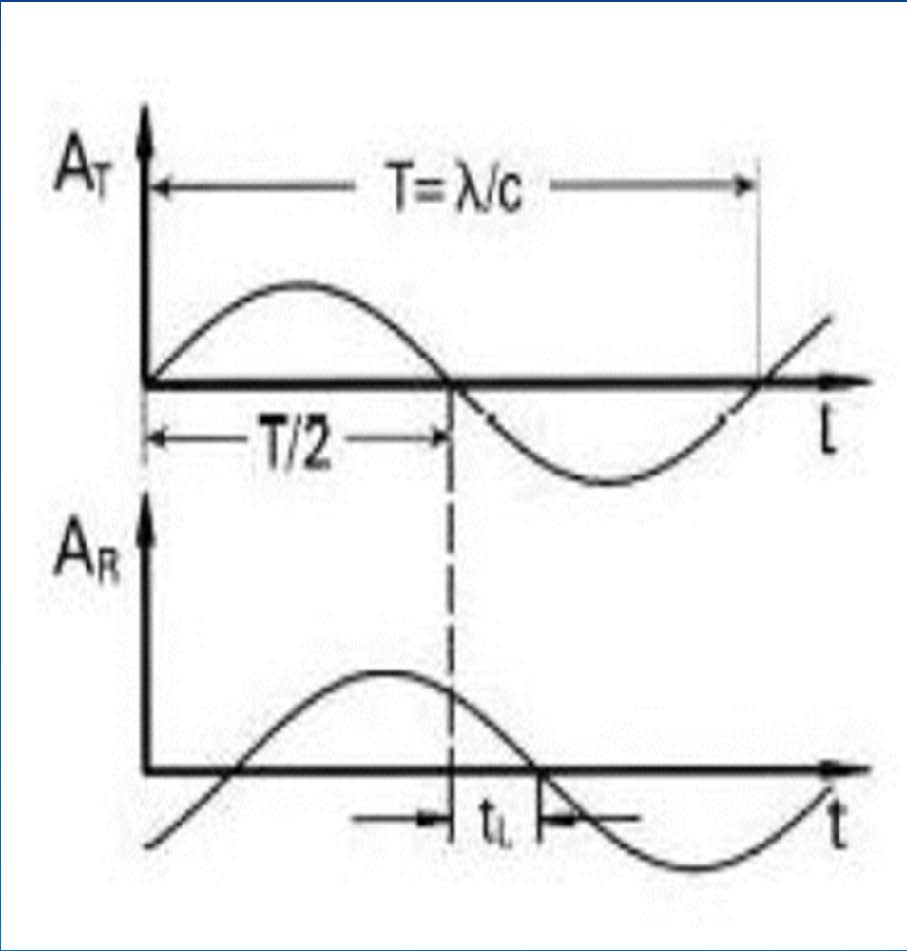
\includegraphics[width=0.5\linewidth,height=0.2\textheight]{figure/Chapter3/连续波相位差测距原理}
			\caption{连续波相位差测距原理}
			\label{fig:连续波相位差测距原理}
		\end{figure}
		
		若在时间$ T $内的被接收的波与被发射波的相位差为$ \varphi $,则从发射到被接收所用时间为
		\begin{equation}
		t_L = \dfrac{\varphi}{2\cpi}\cdot T
		\end{equation}
		
		测量的距离为
		\begin{equation}
		R = \dfrac{1}{2}c \cdot \dfrac{\varphi}{2\cpi}\cdot T = \dfrac{\lambda}{4\cpi}\varphi
		\end{equation}
	
	\item \textbf{测距分辨率}:相位测距中能够准确测量的是一个周期以内的相位差,测距分辨率为
		\begin{equation}
		\Delta R = \dfrac{\lambda_{\text{short}}}{4\cpi}\varphi
		\end{equation}
	\item \textit{整周模糊度}:图中$ t_L $与接收信号与发射信号的相位差成正比。$ t_L $应表示为
		\begin{equation}
		t_L = \dfrac{\varphi}{2\cpi}T+nT
		\end{equation}
		式中,$ n $为激光从发射到接收所走过的距离中的整周数。由于激光波长以微米计,可见$ n $为一个很大的数。由于实际量测的相位差只在之内,实际计算目标到激光器的距离必须计算出整周数$ n $。
	\item \textbf{多测尺频率}:
		若用单一频率测距时是无法确定整周模糊度的值 ,即测距仪存在多值性问题,要解决这一问题,必须采用几个测尺频率测定同一距离。方法:
		\begin{itemize}
			\item 直接多测尺频率:适用于短距离;
			\item 间接多测尺频率:适用于中长距离;
		\end{itemize} % 多测尺频率
	\item \textbf{最大量测距离}:由于相位差的最大量测值为$ 2\cpi $,有
		\begin{equation}
		R_{\max} = \dfrac{1}{4\cpi}\lambda\varphi = \dfrac{\lambda_{\text{long}}}{2}
		\end{equation}
		\begin{itemize}
			\item \textit{最大不模糊距离}:能够准确测量的最大距离,称为最大不模糊距离。
			\item \textbf{双频观测系统}:在采用多频率系统时,由不同频率所对应的波长可兼顾较高的测距分辨率和较大的测量距离。很明显,由最短波长确定了较高的测距分辨率和精度,最长波长确定了最大不模糊距离。
		\end{itemize}
\end{enumerate} % 连续波相位差测距

\paragraph{结论}
\begin{itemize}
	\item 无论是脉冲激光还是连续波激光,在其它条件不变的情况下,最大测距与反射率的平方根和激光功率的平方根成正比。
	\item 要获得较好的测距效果
		\begin{itemize}
			\item \textbf{气候条件}:大气条件十分重要,干、冷和透明的大气条件下,效果最好;
			\item \textbf{时间条件}:夜间最好,最坏的情况是白天阳光强烈;
			\item \textbf{波段选择}:选择大气透过率高的波段;
		\end{itemize}
\end{itemize}

\subsection{测距精度和信噪比} % Subsection	测距精度与信噪比	----------------------------------------
\paragraph{测距精度和信噪比的关系}激光测距系统的测距精度与测距信号的信噪比的平方根成反比,信噪比愈高,测距精度也越高。
\begin{equation}
\sigma \sim \dfrac{1}{\sqrt{S/N}}
\end{equation}

\paragraph{信噪比} 
\begin{itemize}
	\item 信噪比取决于很多因素,如:接收信号功率、信号带宽、背景辐射、探测器响应灵敏度、放大器噪声等。如图\ref{fig:信号参量之间的关系以及对信噪比的影响}所示。
		\begin{figure}
			\centering
			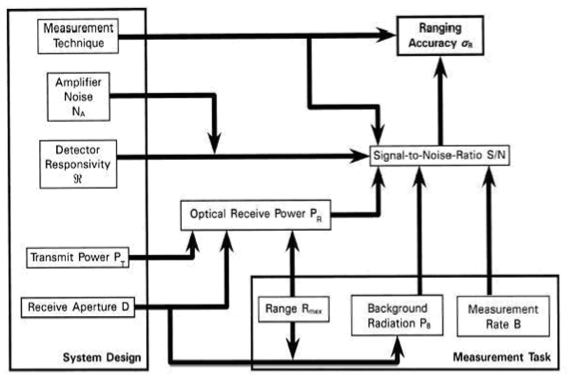
\includegraphics[width=0.7\linewidth]{figure/Chapter3/信号参量之间的关系以及对信噪比的影响}
			\caption{信号参量之间的关系以及对信噪比的影响}
			\label{fig:信号参量之间的关系以及对信噪比的影响}
		\end{figure}
	\item \textbf{信噪比简化}
		\begin{equation}
		S/N = \dfrac{\text{光电二极管电流中的信号功率}}{\text{光电二极管和放大器中的热噪声}}
		\end{equation}
\end{itemize}

\paragraph{两种测距方式的精度}
由于测距精度和信噪比成反比,如果脉冲测距时噪声带宽为$ B_{\text{pulse}} $,相位差测距时噪声带宽为$ B_{\text{cw}} $,则下述关系式成立:
\begin{align}
\sigma_{R_{\text{pulse}}} & \sim \dfrac{c}{2}t_{\text{rise}}\dfrac{\sqrt{B_{\text{pulse}}}}{P_{R_{\text{peak}}}} \\
\sigma_{R_{\text{cw}}} & \sim \dfrac{\lambda_{\text{short}}}{4\cpi}\dfrac{\sqrt{B_{\text{cw}}}}{P_{R_{\text{av}}}}
\end{align}
式中,$ P_{R_{\text{peak}}} $表示脉冲接收功率峰值,$ P_{R_{\text{av}}} $表示连续波接收功率平均值。

假定对同一目标进行量测,可以用发射功率代替接收功率,即以脉冲激光发射功率峰值$ P_{T_{\text{peak}}} $代替接收功率峰值$ P_{R_{\text{peak}}} $,以连续波发射功率平均值$ P_{T_{\text{av}}} $代替接收功率平均值$ P_{R_{\text{av}}} $。于是有:
\begin{equation}\label{equ:两种测距方式精度之比1}
\dfrac{\sigma_{R_{\text{pulse}}}}{\sigma_{R_{\text{cw}}}} \sim 2\cpi \dfrac{c}{\lambda}t_{\text{rise}} \dfrac{P_{T_{\text{av}}}}{P_{T_{\text{peak}}}} \sqrt{\dfrac{B_{\text{pulse}}}{B_{\text{cw}}}}
\end{equation}
假定
\begin{equation}
t_{\text{rise}} \sim \dfrac{1}{B_{\text{pluse}}}
\end{equation}
式\eqref{equ:两种测距方式精度之比1}可以写为
\begin{equation}
\dfrac{\sigma_{R_{\text{pulse}}}}{\sigma_{R_{\text{cw}}}} \sim 2\cpi f \sqrt{\dfrac{t_{\text{rise}}}{B_{\text{cw}}}} \dfrac{P_{T_{\text{av}}}}{P_{T_{\text{peak}}}}
\end{equation}

\paragraph{现状}脉冲激光系统具有大功率、可远距离测距等特点,
目前市场上绝大多数为脉冲激光系统,很少有半导体连续波激光系统。
不过脉冲系统要达到很高的精度需要非常高的技术手段和复杂的处理方法。

\paragraph{测距误差}\textit{测距误差}是指测距仪的显示结果与实际距离之差。
\begin{enumerate}
	\item \textbf{测距误差来源}:噪声、脉冲宽度和幅度、电光系统的延迟以及时间测量单元中基准振荡频率的稳定性。
	\item \textbf{脉冲激光测距仪的误差}
		\begin{itemize}
			\item \textbf{系统误差}:
				\begin{itemize*}
					\item 计数器误差
					\item 大气折射误差
					\item 光电延迟误差
				\end{itemize*}
			\item \textbf{随机误差}:
				\begin{itemize*}
					\item 噪声误差
					\item 距离误差
					\item 漂移误差
				\end{itemize*}
		\end{itemize} % 脉冲激光测距仪的误差
	\item \textbf{连续波激光测距仪测距误差}
		\begin{itemize}
			\item \textbf{固定误差}:
				\begin{itemize*}
					\item 数字测相误差
					\item 幅相误差
					\item 照准误差
				\end{itemize*}
			\item \textbf{比例误差}:
				\begin{itemize*}
					\item 真空光速误差
					\item 大气折射率误差
					\item 测尺频率误差
				\end{itemize*}
		\end{itemize} % 连续波激光测距仪测距误差
	\item \textbf{影响LiDAR测距精度的因素还有}
		\begin{itemize}
			\item 激光功率
			\item 光束发散度
			\item 目标反射特性
			\item 探测器灵敏度
			\item 飞行高度
			\item 飞机姿态
		\end{itemize} % 影响LiDAR测距精度的因素还有
\end{enumerate} % 测距误差

\subsection{功率} % Subsection	功率	----------------------------------------
由于LiDAR系统是在空中对地面进行扫描的,它需要有很高的工作功率,这样才能使激光束的能量尽可能大,经过长距离的大气损耗 和目标吸收等能量损失后,回到探测器时能够有足够的能量,使得探测器能够对光束进行记录。

\paragraph{峰值功率与平均功率}
对于脉冲测距系统,激光能量为:
\begin{equation}
E_{\text{pluse}} = P_{T_{\text{peak}}} t_{\text{pulse}}
\end{equation}
式中,$ t_{\text{pulse}} $为脉冲宽度,$ P_{T_{\text{peak}}} $为发射功率峰值。
	
如果脉冲频率为$ f_{\text{pluse}} $,则平均功率为
\begin{equation}
P_{T_{\text{av}}} = E_{\text{pluse}}f_{\text{pluse}}
\end{equation}

联立求解,得
\begin{equation}
P_{T_{\text{peak}}} = \dfrac{E_{\text{pluse}}}{t_{\text{pulse}}} = \dfrac{P_{T_{\text{av}}}}{t_{\text{pulse}}f_{\text{pluse}}}
\end{equation}
尽管平均功率不大,脉冲激光测距能够产生很高的峰值功率。

\paragraph{发射功率与接受功率}
\begin{equation}
P_r = \rho \dfrac{M^2 A_r}{\cpi R^2} P_T
\end{equation}
式中,$ M $为大气透过率,$ \rho $为目标反射率,$ R $为目标到激光器的距离,$ A_r $为接收光孔截面积。

接受功率的特点:
\begin{itemize}
	\item LiDAR系统接收的功率只是发射功率的很小部分,必须采用非常灵敏的探测器接收信号 。
	\item 接收功率与距离平方成反比
		\begin{itemize}
			\item 激光束刚刚发射出来,由于空中的尘埃或其它的干 扰,会有一部分信号返回接收光路,即使这个部分非常小,也会被灵敏的探测器认为是目标的回波。
			\item 为了避免这种情况,需要采取\textit{近距离消除技术}(close-range suppression techniques)和其它方法。
		\end{itemize}
\end{itemize}

\subsection{体积} % Subsection	体积	----------------------------------------
由于LiDAR系统安装在空中平台上,飞机 的载重量和体积都是有限的,在有限的空间 中需要装载LiDAR设备、操作人员等。
因此,需要将LiDAR设备的体积和重量减小到最小, 这也要求测距仪的体积和重量都很小。

\subsection{波长} % Subsection	波长	----------------------------------------
\paragraph{选择波长的依据}
\begin{itemize}
	\item 大气窗口
	\item 背景光的区别
	\item 目标反射率
	\item 探测器灵敏度
	\item 人眼安全
\end{itemize}

\paragraph{常见LiDAR系统的激光波长} 如表\ref{tab:常见LiDAR系统的激光波长}所示。

\begin{table}[!htbp]
	\centering
	\begin{tabular}{|c|c|}
		\hline
		              系统              &       激光波长       \\ \hline
		\multirow{2}{*}{Leica ALS50II} &  790$ \sim $820  \\ \cline{2-2}
		                               & 1050$ \sim $1060 \\ \hline
		        Optech 3100EA          &       1064       \\ \hline
		      TopoSys FALCON II        &       1560       \\ \hline
		        Riegl LMS-Q560         &       1500       \\ \hline
	\end{tabular}
	\caption{常见LiDAR系统的激光波长}
	\label{tab:常见LiDAR系统的激光波长}
\end{table}

\section{全球定位系统技术} %% Section	全球定位系统技术	========================================
\paragraph{全球定位系统}\textit{全球定位系统}(GPS, Global Position System)是一种利用人造地球卫星进行点位测量导航的技术。
全称是NAVSTAR GPS(NAVigation Satellite Timing And Ranging Global Positioning System)。

\paragraph{GPS定位原理}利用\textbf{测距交会确定点位}。由于用户接受机使用的时钟与卫星星载时钟不可能总是同步,所以除了用户的三维坐标$ (x,y,z) $外,还要引入一个关于卫星与接收机之间的时间差作为未知数$ \delta T $。所以如果想知道解收机所处的位置,至少要能接收到4个卫星的信号。

\paragraph{GPS的组成}
\begin{itemize}
	\item \textbf{空间部分}:GPS卫星星座。如图\ref{fig:GPS星座}所示。
		\begin{itemize}
			\item 由21颗工作卫星和3颗备用卫星组成。
			\item 均匀分布在六个相互夹角为$ 60^{\circ} $的轨道平面内。
			\item GPS卫星用L波段两种频率的无线电波(1575.42 MHz和 1227.6 MHz)向用户发射导航定位信号,同时接收地面发送的导航电文以及调度命令。
		\end{itemize}
		
		\begin{figure}[htbp]
			\centering
			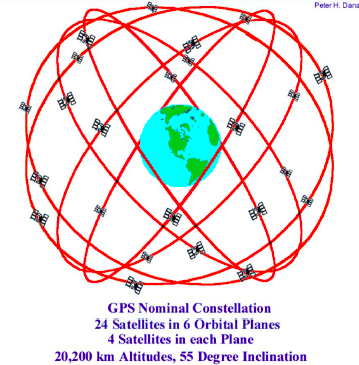
\includegraphics[width=0.5\linewidth]{figure/Chapter3/GPS星座}
			\caption{GPS星座}
			\label{fig:GPS星座}
		\end{figure}
	\item \textbf{地面控制部分}:地面监控系统。
		包括位于美国科罗拉多的主 控站以及分布全球的三个注入站和五个监测站组成,实现对GPS卫星运行的监控。
		主要任务是采集数据(对空中卫星进行连续观测),推算编制各卫星的星历、卫星钟差及大气层的修正参数等,并将这些数据发送到卫星上。
	\item \textbf{用户设备部分}:GPS信号接收机。用来捕获GPS卫星发射的信号,并进行处理,
		根据信号到达接收机的时间,确定接收机到卫星的距离,并最终确定接收机的精确位置。
\end{itemize} %. GPS的组成

\paragraph{GPS的优点}
\begin{itemize}
	\item 观测站之间无需通视
	\item 定位精度高
	\item 操作简便
	\item 全天候作业
	\item 实时定位速度快
	\item 抗干扰性能好,保密性强
\end{itemize}

\paragraph{GPS定位分类}
\begin{enumerate}
	\item \textbf{按定位方式}
		\begin{itemize}
			\item \textit{单点定位(绝对定位)}:采用一台接收机进行定位的模式。只能采用伪距观测量进行概略导航定位,定位精度较差。
			\item \textit{差分定位(相对定位)}:差分GPS(Differential Global Position System,DGPS)
				在用户接收机附近设置一个坐标已知的差分基准站, 连续接收GPS导航信号,将测得的位置或距离数据与已知的位置、距离数据进行比较,
				确定误差,得出改正值,然后将改正数发播给覆盖区域内的用户,用以改正用户的定位结果。
		\end{itemize} % 按定位方式
	\item \textbf{根据定位所采用的观测值} 
		\begin{itemize*}
			\item 测距码伪距GPS定位
			\item 载波相位GPS定位
		\end{itemize*}
	\item \textbf{根据获取定位结果的时间} 
		\begin{itemize*}
			\item 实时GPS定位
			\item 非实时GPS定位
		\end{itemize*}
	\item \textbf{根据定位时接收机的运动状态} 
		\begin{itemize*}
			\item 动态GPS定位
			\item 静态GPS定位
		\end{itemize*}
\end{enumerate}

\paragraph{GPS精度影响因素}
\begin{itemize}
	\item 接收机公有的误差
	\item 传播延迟误差
	\item 接收机固有的误差
\end{itemize}
DGPS技术可以完全消除第一部分误差,大部分消除第二部分误差(取决于基准站和流动站之间的距离)。

\paragraph{LiDAR系统的GPS技术}
LiDAR系统要求很高的定位精度,采取的是载波相位 差分GPS技术,又称为RTK(Real Time Kinematic)技术,
建立在实时处理两个测站的载波相位观测值的基础上,它能实时提供观测点的三维坐标,可以达到厘米级的高精度。

由于涉及到测定遥感器投影中心的位置方位元素,在机载激光雷达系统中,GPS动态定位的精度成为影响系统精度的主要因素。
一般而言,LiDAR系统上使用的载 波相位差分GPS定位精度在5 cm$ \sim $10 cm。

\paragraph{LiDAR系统中GPS的作用}
\begin{itemize}
	\item 确定成像时刻系统中心的地理坐标
	\item 提供相关数据给姿态测量装置,提高测定姿态角的测角精度
	\item 提供导航控制数据
\end{itemize}

\section{惯性测量系统技术} %% Section	全球定位系统技术	========================================
\subsection{惯性导航系统} % Subsection	惯性导航系统	----------------------------------------
\paragraph{基本原理}
\textit{惯性导航系统}(Inertial Navigation System, INS),利用陀螺和加速度计等惯性元件测量运行体在运动过程中的旋转角速度和加速度,计算得到运动体的相对位置、速度和姿态等导航参数。
结构如图\ref{fig:惯性导航系统结构}所示。

\begin{figure}[htbp]
	\centering
	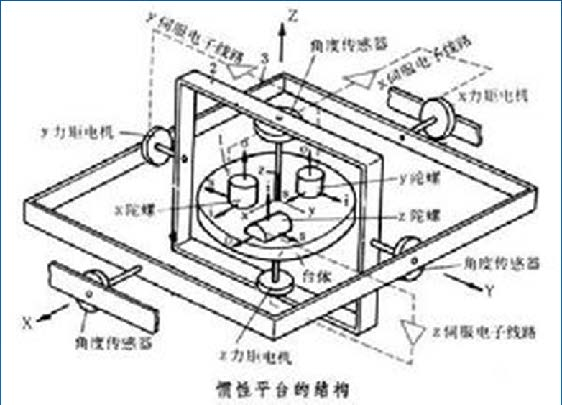
\includegraphics{figure/Chapter3/惯性导航系统结构}
	\caption{惯性导航系统结构}
	\label{fig:惯性导航系统结构}
\end{figure}

\paragraph{作用}可以用于定位、测速、输出姿态信息,以及测定重力异常和垂线偏差、相对大地水准面起伏等。

\paragraph{惯性测量单元} 惯性导航系统中负责姿态测定的陀螺和加速度计等惯性元件总称为\textit{惯性测量单元}(Inertial Measurement Unit, IMU),它是INS的核心部件。IMU通常由三个加速度计和三个陀螺、数字电路和CPU组成的。

\subsection{IMU与DGPS组合定位技术} % Subsection	IMU与DGPS组合定位技术	----------------------------------------
\paragraph{DGPS技术的特点}
\begin{itemize}
	\item \textbf{优点}:使用方便、成本低廉,可量测传感器的位置和速率,高精度、误差不随时间积累。
	\item \textbf{缺点}:动态性能差、数据输出频率低(易受到干扰而失锁),无法量测瞬间的快速变化,没有姿态量测功能等。
\end{itemize}

\paragraph{IMU技术的特点}
\begin{itemize}
	\item \textbf{优点}:姿态量测功能,具有完全自主、无信号传播,既能定位、测速,又可快速量测传感器瞬间的移动,输出姿态信息。
	\item \textbf{缺点}:位误差随着时间迅速积累增长,每次使用前初始对准时间长,不能长时间单独工作,必须不断加以校准。
\end{itemize}

\paragraph{POS系统}GPS技术+IMU技术
\begin{itemize}
	\item 提高了定位精度
	\item 增强了系统可靠性
	\item 部分解决了采样频率低的问题
\end{itemize}

\section{高性能二维扫描技术} %% Section	全球定位系统技术	========================================
\subsection{机载LiDAR系统四种典型的扫描方式} % Subsection	机载LiDAR系统四种典型的扫描方式	----------------------------------------
\begin{enumerate}
	\item \textit{摆镜扫描}:通过电机带动反射镜反复摆动一定的角度,实现激光束在地面的扫描。扫描原理和脚点形状如图\ref{fig:摆镜扫描}所示。
		\begin{figure}[htbp]
			\centering
			\begin{subfigure}[t]{0.3\linewidth}
				\centering
				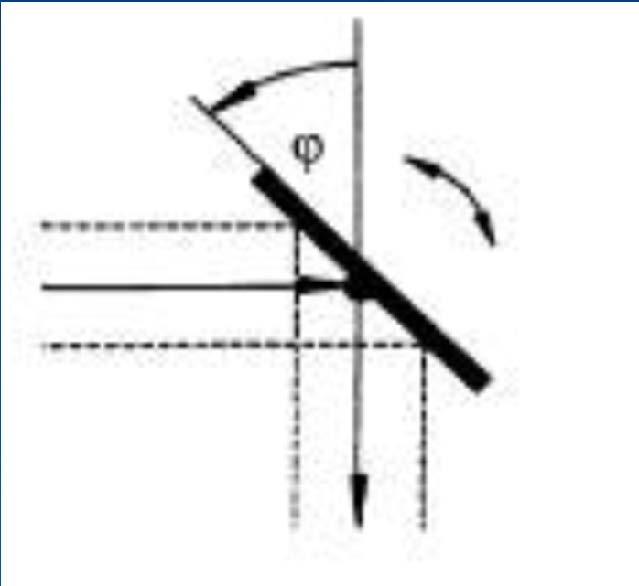
\includegraphics[height=3cm]{figure/Chapter3/摆镜扫描1}
				\subcaption{摆镜扫描原理}
			\end{subfigure}
			\begin{subfigure}[t]{0.3\linewidth}
				\centering
				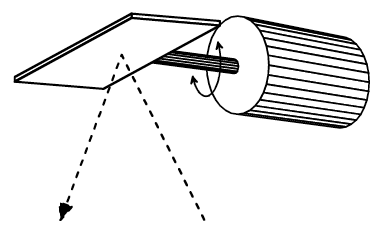
\includegraphics[height=3cm]{figure/Chapter3/摆镜扫描2}
				\subcaption{摆镜扫描结构}
			\end{subfigure}
			\begin{subfigure}[t]{0.3\linewidth}
				\centering
				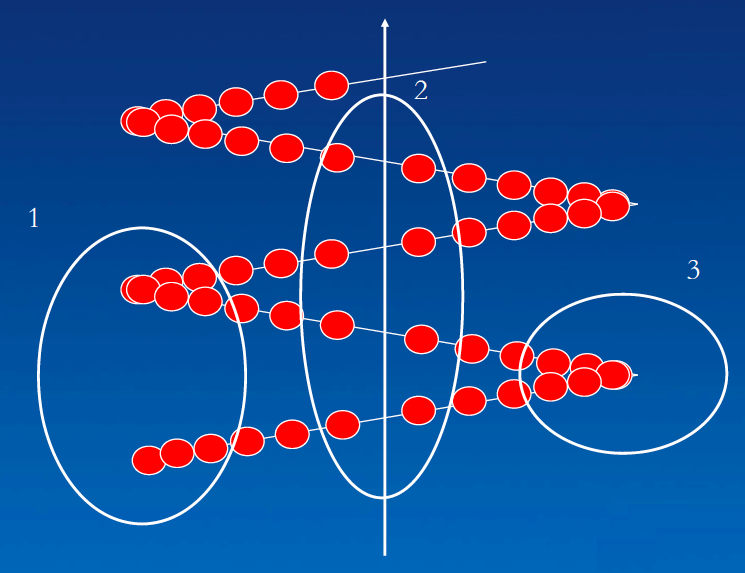
\includegraphics[height=3cm]{figure/Chapter3/摆镜扫描_脚点}
				\subcaption{摆镜扫描脚点}
			\end{subfigure}
			\caption{摆镜扫描}
			\label{fig:摆镜扫描}
		\end{figure}
	\item \textit{旋转棱镜扫描}:通过电机带动多面棱镜旋转,由于镜面的位置在不断变化,导致反射光束的方向在一定的范围内往复变化,从而实现激光束在地面的扫描。如图\ref{fig:旋转棱镜扫描}所示。
		\begin{figure}[htbp]
			\centering
			\begin{subfigure}[t]{0.45\linewidth}
				\centering
				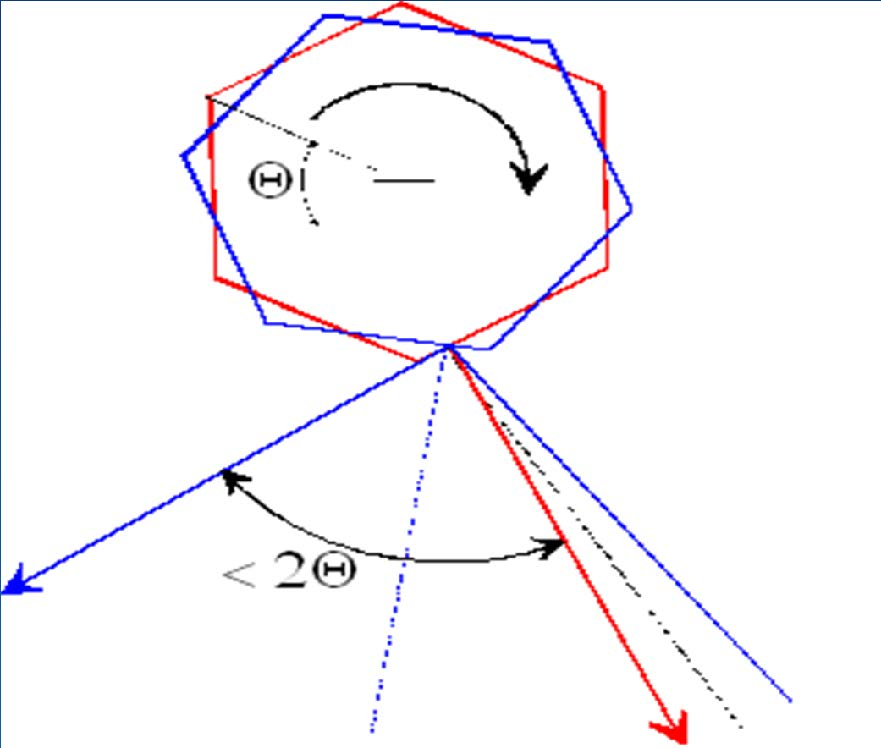
\includegraphics[height=3cm]{figure/Chapter3/旋转棱镜扫描原理}
				\subcaption{旋转棱镜扫描原理}
			\end{subfigure}
			\begin{subfigure}[t]{0.45\linewidth}
				\centering
				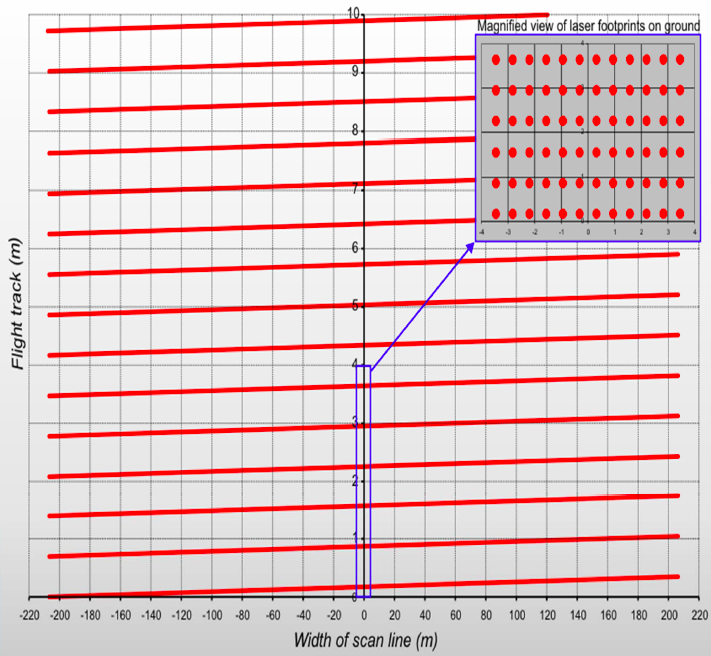
\includegraphics[height=3cm]{figure/Chapter3/旋转棱镜扫描脚点形状}
				\subcaption{旋转棱镜扫描脚点形状}
			\end{subfigure}
			\caption{旋转棱镜扫描}
			\label{fig:旋转棱镜扫描}
		\end{figure}
	\item \textit{椭圆扫描}:旋转一周后在地面形成椭圆扫线。如图\ref{fig:椭圆扫描}所示。
		\begin{figure}[htbp]
			\centering
			\begin{subfigure}[t]{0.3\linewidth}
				\centering
				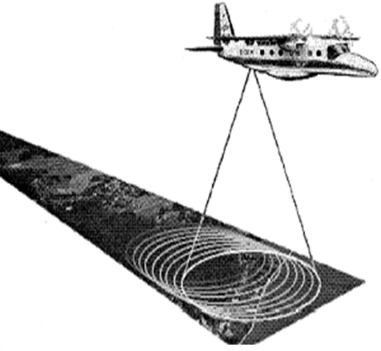
\includegraphics[height=3cm]{figure/Chapter3/椭圆扫描1}
				\subcaption{椭圆扫描示意图}
			\end{subfigure}
			\begin{subfigure}[t]{0.3\linewidth}
				\centering
				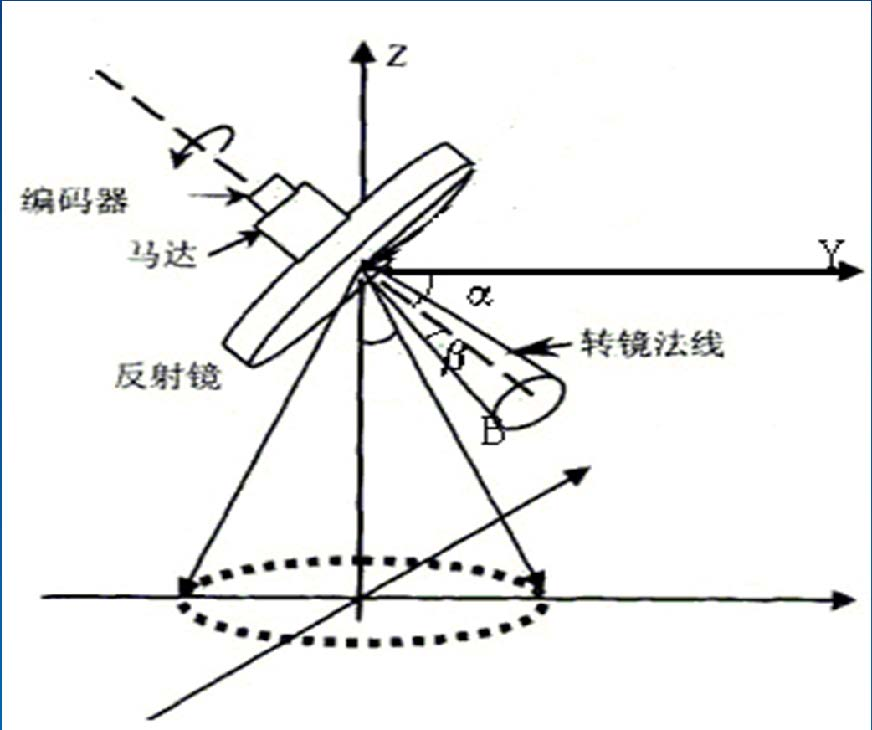
\includegraphics[height=3cm]{figure/Chapter3/椭圆扫描2}
				\subcaption{椭圆扫描原理}
			\end{subfigure}
			\begin{subfigure}[t]{0.3\linewidth}
				\centering
				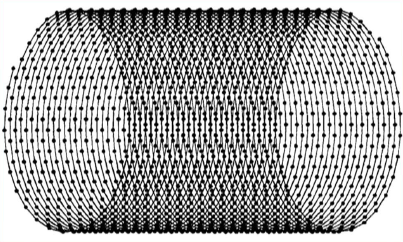
\includegraphics[height=3cm]{figure/Chapter3/椭圆扫描脚点形状}
				\subcaption{椭圆扫描脚点形状}
			\end{subfigure}
			\caption{椭圆扫描}
			\label{fig:椭圆扫描}
		\end{figure}
	\item \textit{光纤扫描}:如图\ref{fig:光纤扫描}所示。目前仅TopoSys激光系统采用光纤扫描仪。目前已有128根光纤组,256根光纤组将可以实现。
		\begin{figure}[htbp]
			\centering
			\begin{subfigure}[t]{0.45\linewidth}
				\centering
				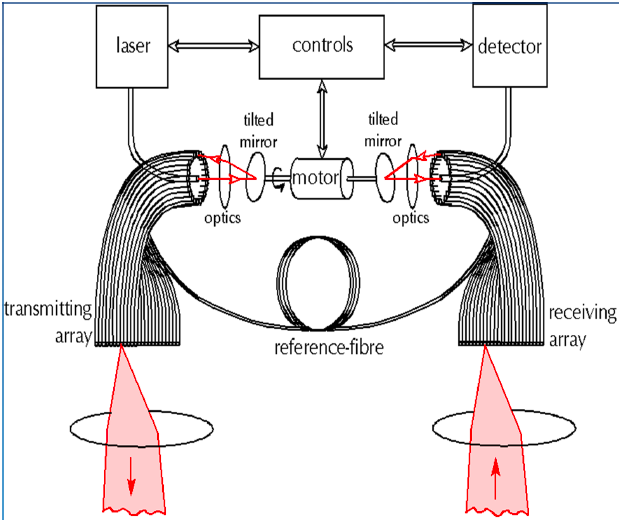
\includegraphics[height=3cm]{figure/Chapter3/光纤扫描原理}
				\subcaption{光纤扫描原理}
			\end{subfigure}
			\begin{subfigure}[t]{0.45\linewidth}
				\centering
				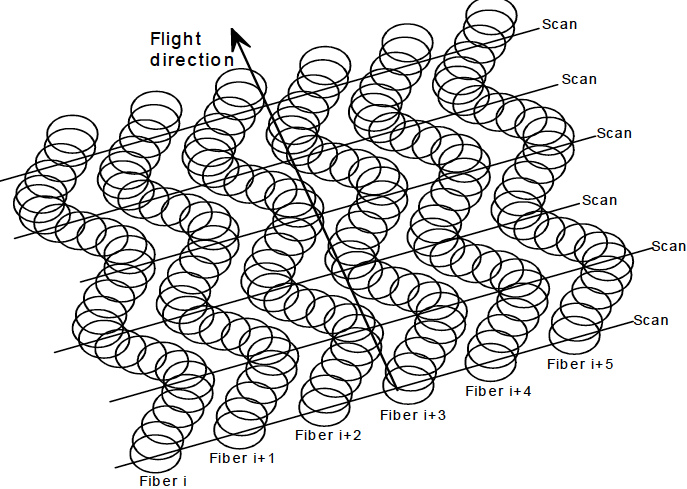
\includegraphics[height=3cm]{figure/Chapter3/光纤扫描脚点}
				\subcaption{光纤扫描脚点}
			\end{subfigure}
			\caption{光纤扫描}
			\label{fig:光纤扫描}
		\end{figure}
\end{enumerate} % 机载LiDAR系统四种典型的扫描方式

\subsection{扫描线形状} % Subsection	扫描线形状	----------------------------------------
扫描线在地面形成的形状不仅取决于激光扫描装置及其工作方式,也取决于飞行方向、飞行速度和地形。

沿着扫描方向对地面目标的连续扫描,是一种等角度步进扫 ,激光所照射的那些点并不是等间距的。由于有时扫 速度不平衡,或加快或减慢,造成扫 线边上的点出现异样,表现出不同的特征,有时就需要从所采集的数据集合中去除这些点。

\paragraph{分类}
\begin{enumerate}
	\item \textbf{按扫描方式}:摆镜扫描;旋转棱镜扫描;椭圆扫描;光纤扫描。
	\item \textbf{按激光扫描方向}:单向扫描;双向扫描。
	\item \textbf{按扫描轨迹}:线扫描;椭圆扫描。
\end{enumerate}

\section{LiDAR数据获取处理}

\paragraph{机载LiDAR获取的数据}
\begin{itemize}
	\item 距离数据、强度信息、CCD等遥感数据
	\item DGPS系统及INS系统等定位定姿数据、航迹文件
	\item 激光点分布模式与技术数据等辅助数据
\end{itemize}
这些信息数据必须通过同步信号,保持相互关联、匹配,才能使用!

\subsection{离线时间同步方案}如图\ref{fig:离线时间同步方案}所示。
\begin{itemize}
	\item POS数据和激光扫描数据存储在不同PC机硬盘中。
	\item POS数据与GPS时间相关,激光扫描数据与PC1的计算机内部时间相关。
	\item PC1与PC2借助GPS的PPS信号关联。
\end{itemize}
\begin{figure}[htbp]
	\centering
	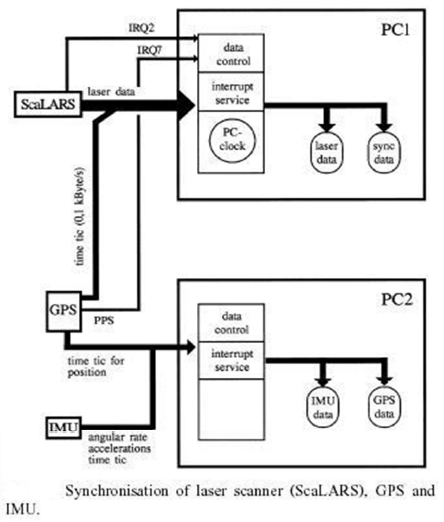
\includegraphics[width=0.5\linewidth]{figure/Chapter3/离线时间同步方案}
	\caption{离线时间同步方案}
	\label{fig:离线时间同步方案}
\end{figure}

\subsection{机载LiDAR系统对地定位方程}

\paragraph{摆镜扫描对地定位方程}通过激光对地面的扫描得到扫描仪与地面上各点的距离,由GPS接收机得到扫描仪的位置,由高精度姿态量测装置量测出扫描仪的姿态,即$ φ $、$ ω $、$ κ $角度,由这些量测值可计算出地面点的三维坐标。

设地面点$ P $在地面坐标系中的坐标为$ (X,Y,Z)_p $, $ P $在传感器坐标系中的坐标为$ (U,V,W)_P $,投影中心$ S $在地面坐标系中的坐标为$ (X_S,Y_S,Z_S) $,传感器的姿态角为$ (\varphi,\omega,\kappa) $,则通用的构象方程为
\begin{equation}
\begin{pmatrix}
X \\ Y \\ Z
\end{pmatrix}_P = \begin{pmatrix}
X_S \\ Y_S \\ Z_S
\end{pmatrix} + \symbf{A} \begin{pmatrix}
U \\ V \\ W
\end{pmatrix}_P
\end{equation}
其中,
\begin{equation}
\symbf{A} = \begin{pmatrix}
a_1 & a_2 & a_3 \\
b_1 & b_2 & b_3 \\
c_1 & c_2 & c_3 
\end{pmatrix}
\end{equation}
是传感器坐标系相对于地面坐标系的旋转矩阵,是传感器姿态角的函数。

对于每一个脉冲,有
\begin{align}
	\begin{split}
	x & = 0 \\
	y & = S \sin \theta \\
	z & = S \cos \theta
	\end{split}
\end{align}
式中,$ \theta $是扫描线方向与$ Z $轴夹角,由编码器按固定的激光脉冲间隔给出;$ S $是激光测距。

代入构像方程,有扫描线定位方程
\begin{equation}
\begin{pmatrix}
X \\ Y \\ Z
\end{pmatrix}_P = \begin{pmatrix}
X_S \\ Y_S \\ Z_S
\end{pmatrix} + \symbf{A} \begin{pmatrix}
0 \\ S\sin\theta \\ S\cos\theta
\end{pmatrix}_P
\end{equation}

\paragraph{椭圆扫描定位方程}
\begin{equation}
\begin{pmatrix}
X_P \\ Y_P \\ Z_P
\end{pmatrix} = \begin{pmatrix}
X_G \\ Y_G \\ Z_G
\end{pmatrix} + \symbf{A} \begin{pmatrix}
-S\sin 2\delta \sin \gamma \\ 
S \cos 2\delta \\ 
-S \sin 2\delta \cos \gamma
\end{pmatrix}
\end{equation}

\section{机载LiDAR数据获取新技术} %% Section	全球定位系统技术	========================================
\paragraph{数字化全波形技术}如图\ref{fig:数字化全波形技术}所示。
\begin{figure}[htbp]
	\centering
	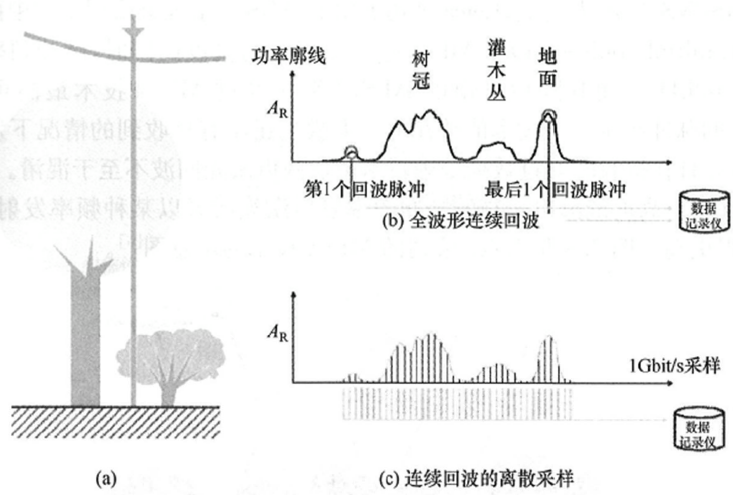
\includegraphics[width=0.7\linewidth]{figure/Chapter3/数字化全波形技术}
	\caption{数字化全波形技术}
	\label{fig:数字化全波形技术}
\end{figure}

\paragraph{空中内插多脉冲技术}如图\ref{fig:空中内插多脉冲技术}所示。
\begin{figure}[htbp]
	\centering
	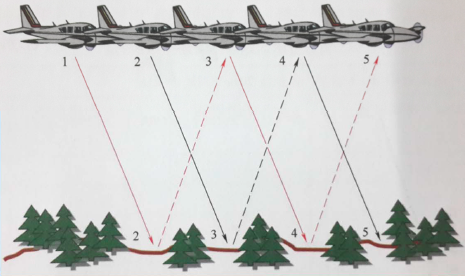
\includegraphics[width=0.7\linewidth]{figure/Chapter3/空中内插多脉冲技术}
	\caption{空中内插多脉冲技术}
	\label{fig:空中内插多脉冲技术}
\end{figure}

\paragraph{双扫描仪组合技术}如图\ref{fig:双扫描仪组合技术}所示。
增加地面激光脚点密度的方法:
\begin{itemize}
	\item 直接的方法就是增大激光脉冲的重复频率和扫描仪的扫描频率。
	\item 多脉冲技术可以通过增加激光脉冲的重复频率来达到这个目的,但是扫描仪的扫描频率由于各方面的限制很难有大幅度的提升。
	\item 双激光雷达组合的系统便应运而生。通过搭载两个激光扫描仪,并使其同时工作,可显著提高地面激光脚点密度。
\end{itemize}

\begin{figure}[htbp]
	\centering
	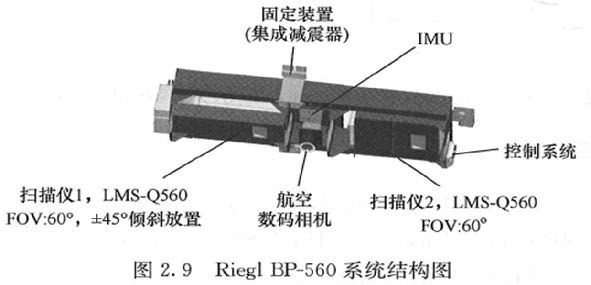
\includegraphics[width=0.7\linewidth]{figure/Chapter3/双扫描仪组合技术}
	\caption{双扫描仪组合技术}
	\label{fig:双扫描仪组合技术}
\end{figure}